
In this section we provide a taxonomy of common failure modes observed in
software-defined networks. We base our analysis on conversations with
researchers at Nicira~\cite{nicira}, a startup focused on developing a network operating
system for production SDN deployments~\cite{onix}.

\begin{figure}[t]
    \centering
    \begin{tabular}{ccc}
    \hspace{-5pt}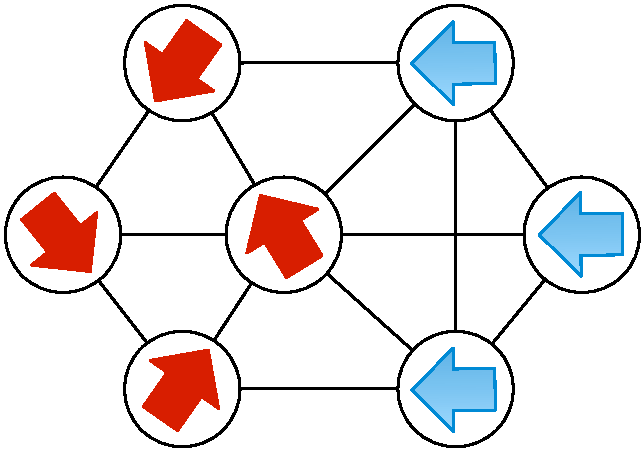
\includegraphics[width=1.3in]{../diagrams/bugs/loop.pdf}&
    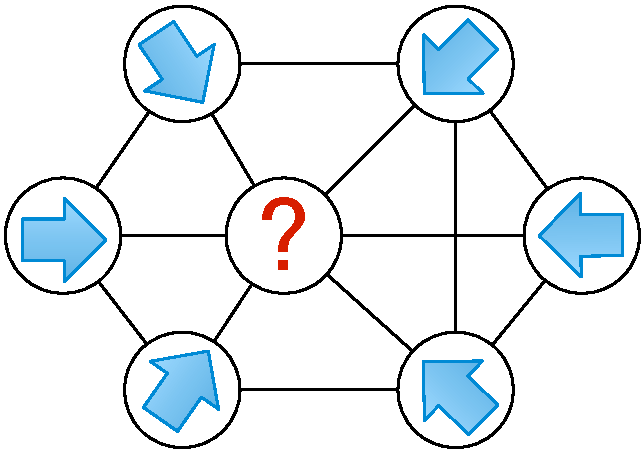
\includegraphics[width=1.3in]{../diagrams/bugs/dead_end.pdf}& \\
    {\bf (i) Loop}&{\bf (ii) Dead End}& \\
    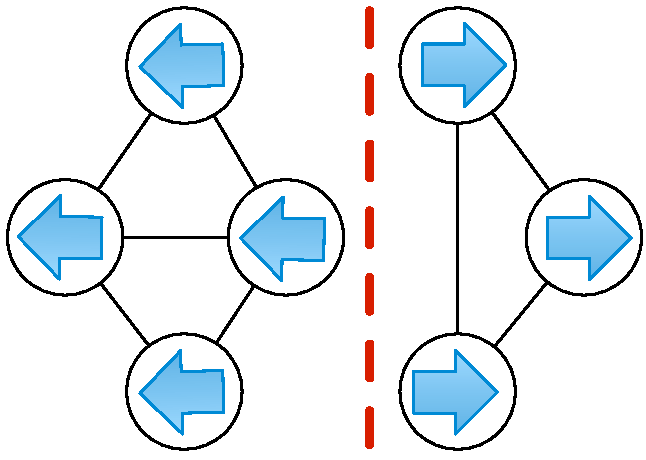
\includegraphics[width=1.3in]{../diagrams/bugs/partition.pdf}&
    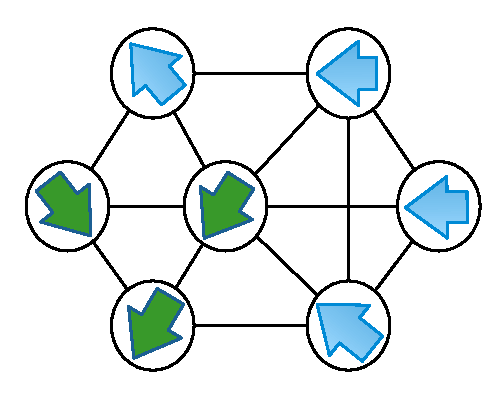
\includegraphics[width=1.3in]{../diagrams/bugs/routing_inconsistency.pdf}\\
     {\bf (iii) Partition}&{\bf (iv) Inconsistency}
    \end{tabular}
    \caption[]{\label{fig:generic_errors} Generic errors observed in
    networks.\vspace{-10pt}} 
\end{figure}


Figure \ref{fig:generic_errors} depicts such
errors. 
Well, loops are these things where packets go in a circle and never come out.
Their bad because they cause the traffic stuck in the loop to never go
through. They're also bad because they congest the routers in the loop, and
therefore affect unrelated traffic. Really bad at layer 2, where there are no
ttls.


Blackholes are a related problem. Traffic may arrive at a dead end,

Maybe talk about routing consistency? Simplest invariant is `No packet can
arrive at a web server without passing through a firewall`. If re-distributing
load across ingress switches, in-flight packets might get the web server
without passing through a firewall.

We note that some error conditions may not manifest themselves in the same way
as a normal network. Network partitions for example. Most OpenFlow networks
don't keep default routes -- the FIBs are sparse. By checking the FIBs alone,
you won't find .

Ok, now for the interesting bugs. Start with Justine's flow overlap bug.

Then go on to virtualization bugs. These are pretty severe, by the way.
Semantic mismatches, yahdah yahdah.

Then consistency. 9 in 10 systems researchers agree, PAXOS is hard.

